%!TEX root = ../dokumentation.tex



\chapter{Benutzeroberfläche}\label{cha:Benutzeroberfläche}
Im folgenden sind Mockups zu sehen, die die zu entwickelnde App darstellen.
Folgende Bildschirme werden hier dargestellt:
\begin{itemize}
	\item Menü
	\item Menü Pop-Up
	\item Flug starten
	\item Flugrouten
	\item Messprofile
	\item Messwerte anzeigen (Karte)
	\item Messwerte anzeigen (Tabelle)
\end{itemize}

\begin{figure}
	\centering
	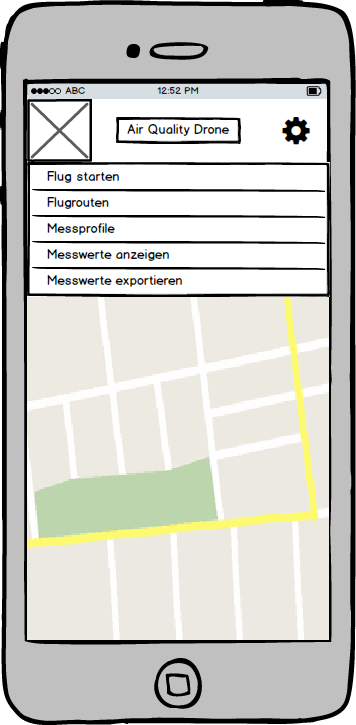
\includegraphics[scale=0.8]{images/Menue}
	\caption{Menü}
\end{figure}
\newpage

\begin{figure}
	\centering
	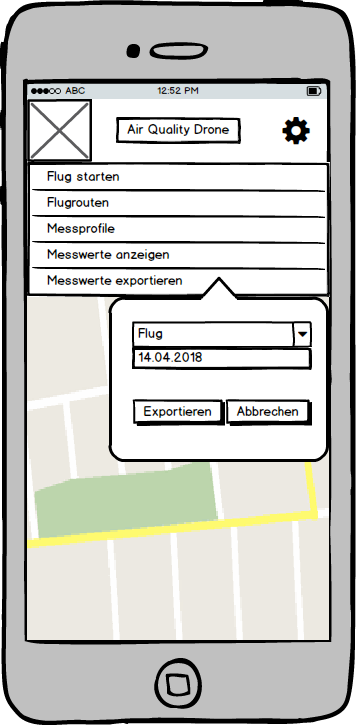
\includegraphics[scale=0.8]{images/MenuePopUp}
	\caption{Menü Pop-Up}
\end{figure}
\newpage

\begin{figure}
	\centering
	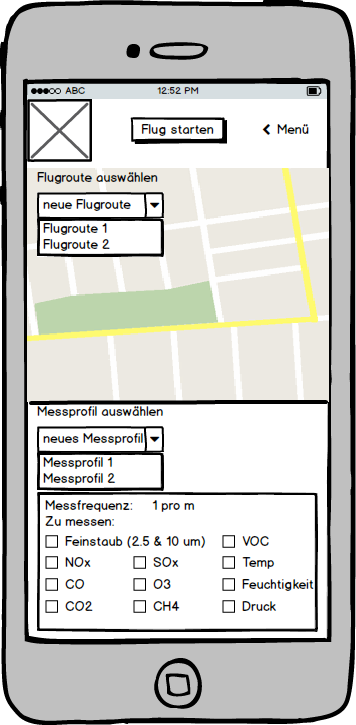
\includegraphics[scale=0.8]{images/FlugStarten}
	\caption{Flug starten}
\end{figure}
\newpage

\begin{figure}
	\centering
	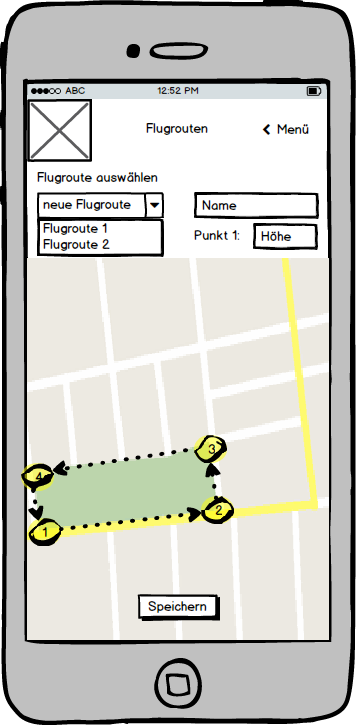
\includegraphics[scale=0.8]{images/Flugrouten}
	\caption{Flugrouten}
\end{figure}
\newpage

\begin{figure}
	\centering
	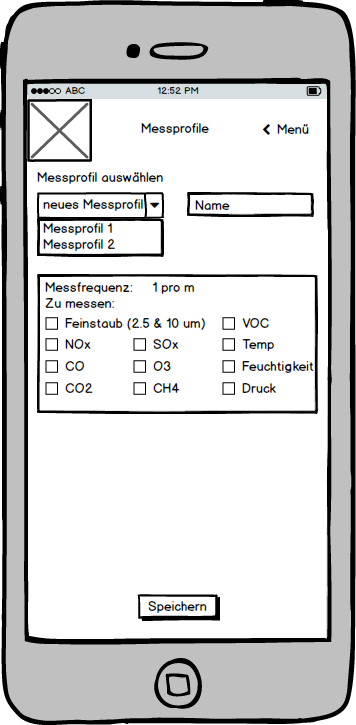
\includegraphics[scale=0.8]{images/Messprofile}
	\caption{Messprofile}
\end{figure}
\newpage

\begin{figure}
	\centering
	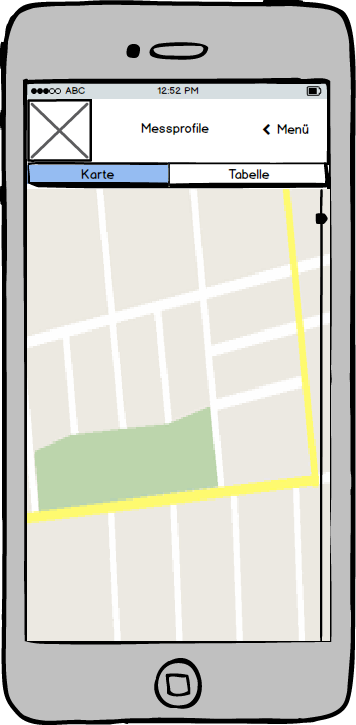
\includegraphics[scale=0.8]{images/MesswerteAnzeigenKarte}
	\caption{Messwerte anzeigen (Karte)}
\end{figure}
\newpage

\begin{figure}
	\centering
	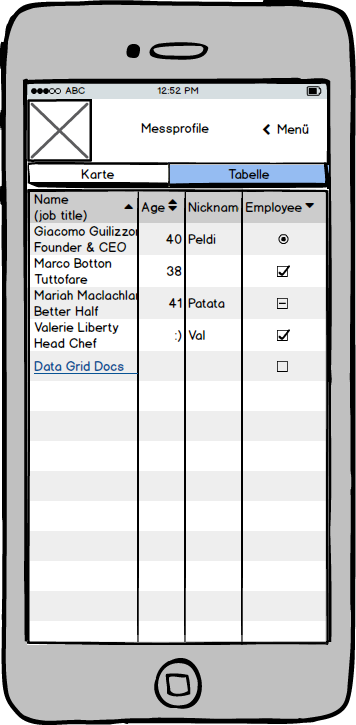
\includegraphics[scale=0.8]{images/MesswerteAnzeigenTabelle}
	\caption{Messwerte anzeigen (Tabelle)}
\end{figure}
\newpage